\documentclass{beamer}

\usefonttheme{professionalfonts} % using non standard fonts for beamer
\usefonttheme{serif} % default family is serif

\usepackage{hyperref}
%\usepackage{minted}
\usepackage{animate}
\usepackage{graphicx}
\def\Put(#1,#2)#3{\leavevmode\makebox(0,0){\put(#1,#2){#3}}}
\usepackage{colortbl}
\usepackage{tikz}
\usepackage{amssymb}
\usepackage{enumerate}
\usepackage{arydshln}
\usepackage{algorithm}
\usepackage{algpseudocode}

\colorlet{lightred}{red!25}
\colorlet{lightgreen}{green!25}


\newcommand\blfootnote[1]{%

  \begingroup

  \renewcommand\thefootnote{}\footnote{#1}%

  \addtocounter{footnote}{-1}%

  \endgroup

}

\makeatletter

%%%%%%%%%%%%%%%%%%%%%%%%%%%%%% Textclass specific LaTeX commands.

 % this default might be overridden by plain title style

 \newcommand\makebeamertitle{\frame{\maketitle}}%

 % (ERT) argument for the TOC

 \AtBeginDocument{%

   \let\origtableofcontents=\tableofcontents

   \def\tableofcontents{\@ifnextchar[{\origtableofcontents}{\gobbletableofcontents}}

   \def\gobbletableofcontents#1{\origtableofcontents}

 }

%%%%%%%%%%%%%%%%%%%%%%%%%%%%%% User specified LaTeX commands.

\usetheme{Malmoe}

% or ...

\useoutertheme{infolines}

\addtobeamertemplate{headline}{}{\vskip2pt}

\setbeamercovered{transparent}

% or whatever (possibly just delete it)

\makeatother

\begin{document}
\title[PFLOCK report]{PFLOCK Report}
\author[AC]{Andres Calderon}
\institute[Spring'20]{University of California, Riverside}
\makebeamertitle
\newif\iflattersubsect

\AtBeginSection[] {
    \begin{frame}<beamer>
    \frametitle{Outline} 
    \tableofcontents[currentsection]  
    \end{frame}
    \lattersubsectfalse
}

\AtBeginSubsection[] {
    \begin{frame}<beamer>
    \frametitle{Outline} 
    \tableofcontents[currentsubsection]  
    \end{frame}
}

\begin{frame}{Solving issues in local quadtree creation}
    \begin{itemize}
        \item The GeoSpark Quadtree library receives three parameters: maximum items per node (capacity), a fraction of the total size of the input to extract a sample (fraction), and a number of levels to limit the depth of the tree (levels). 
        \item I fixed a bug which set incorrectly the value of levels.  It keeps a default value of 8 which allows up to $4^8=64563$ possible leaves.
        \item As we expect relatively small partitions, I have set this value to 5 (no more than 1024 leaves per partition).
    \end{itemize}
\end{frame}

\begin{frame}{Solving issues in local quadtree creation}
    \begin{itemize}
        \item Follows a similar strategy on GeoSpark repository\footnote{\url{https://tinyurl.com/y8fy4ys7}}$^,$\footnote{\url{https://tinyurl.com/ycsb29gz}} to create global quadtrees.
        \item Given a number of desired subgrids (x) and a input size (n):
        \begin{itemize}
            \item capacity = n / x
            \item fraction = a scaled value between 1 (for n < 1000) and 0.01 (for n > 10000)
        \end{itemize}
        \item It works but with a fixed number of subgrids balancing can be a problem...
    \end{itemize}
\end{frame}

\begin{frame}{Example}
    \centering
    
\includegraphics[width=\textwidth]{figures/ByP_Globals}
\end{frame}
\begin{frame}{Example}
    \centering
    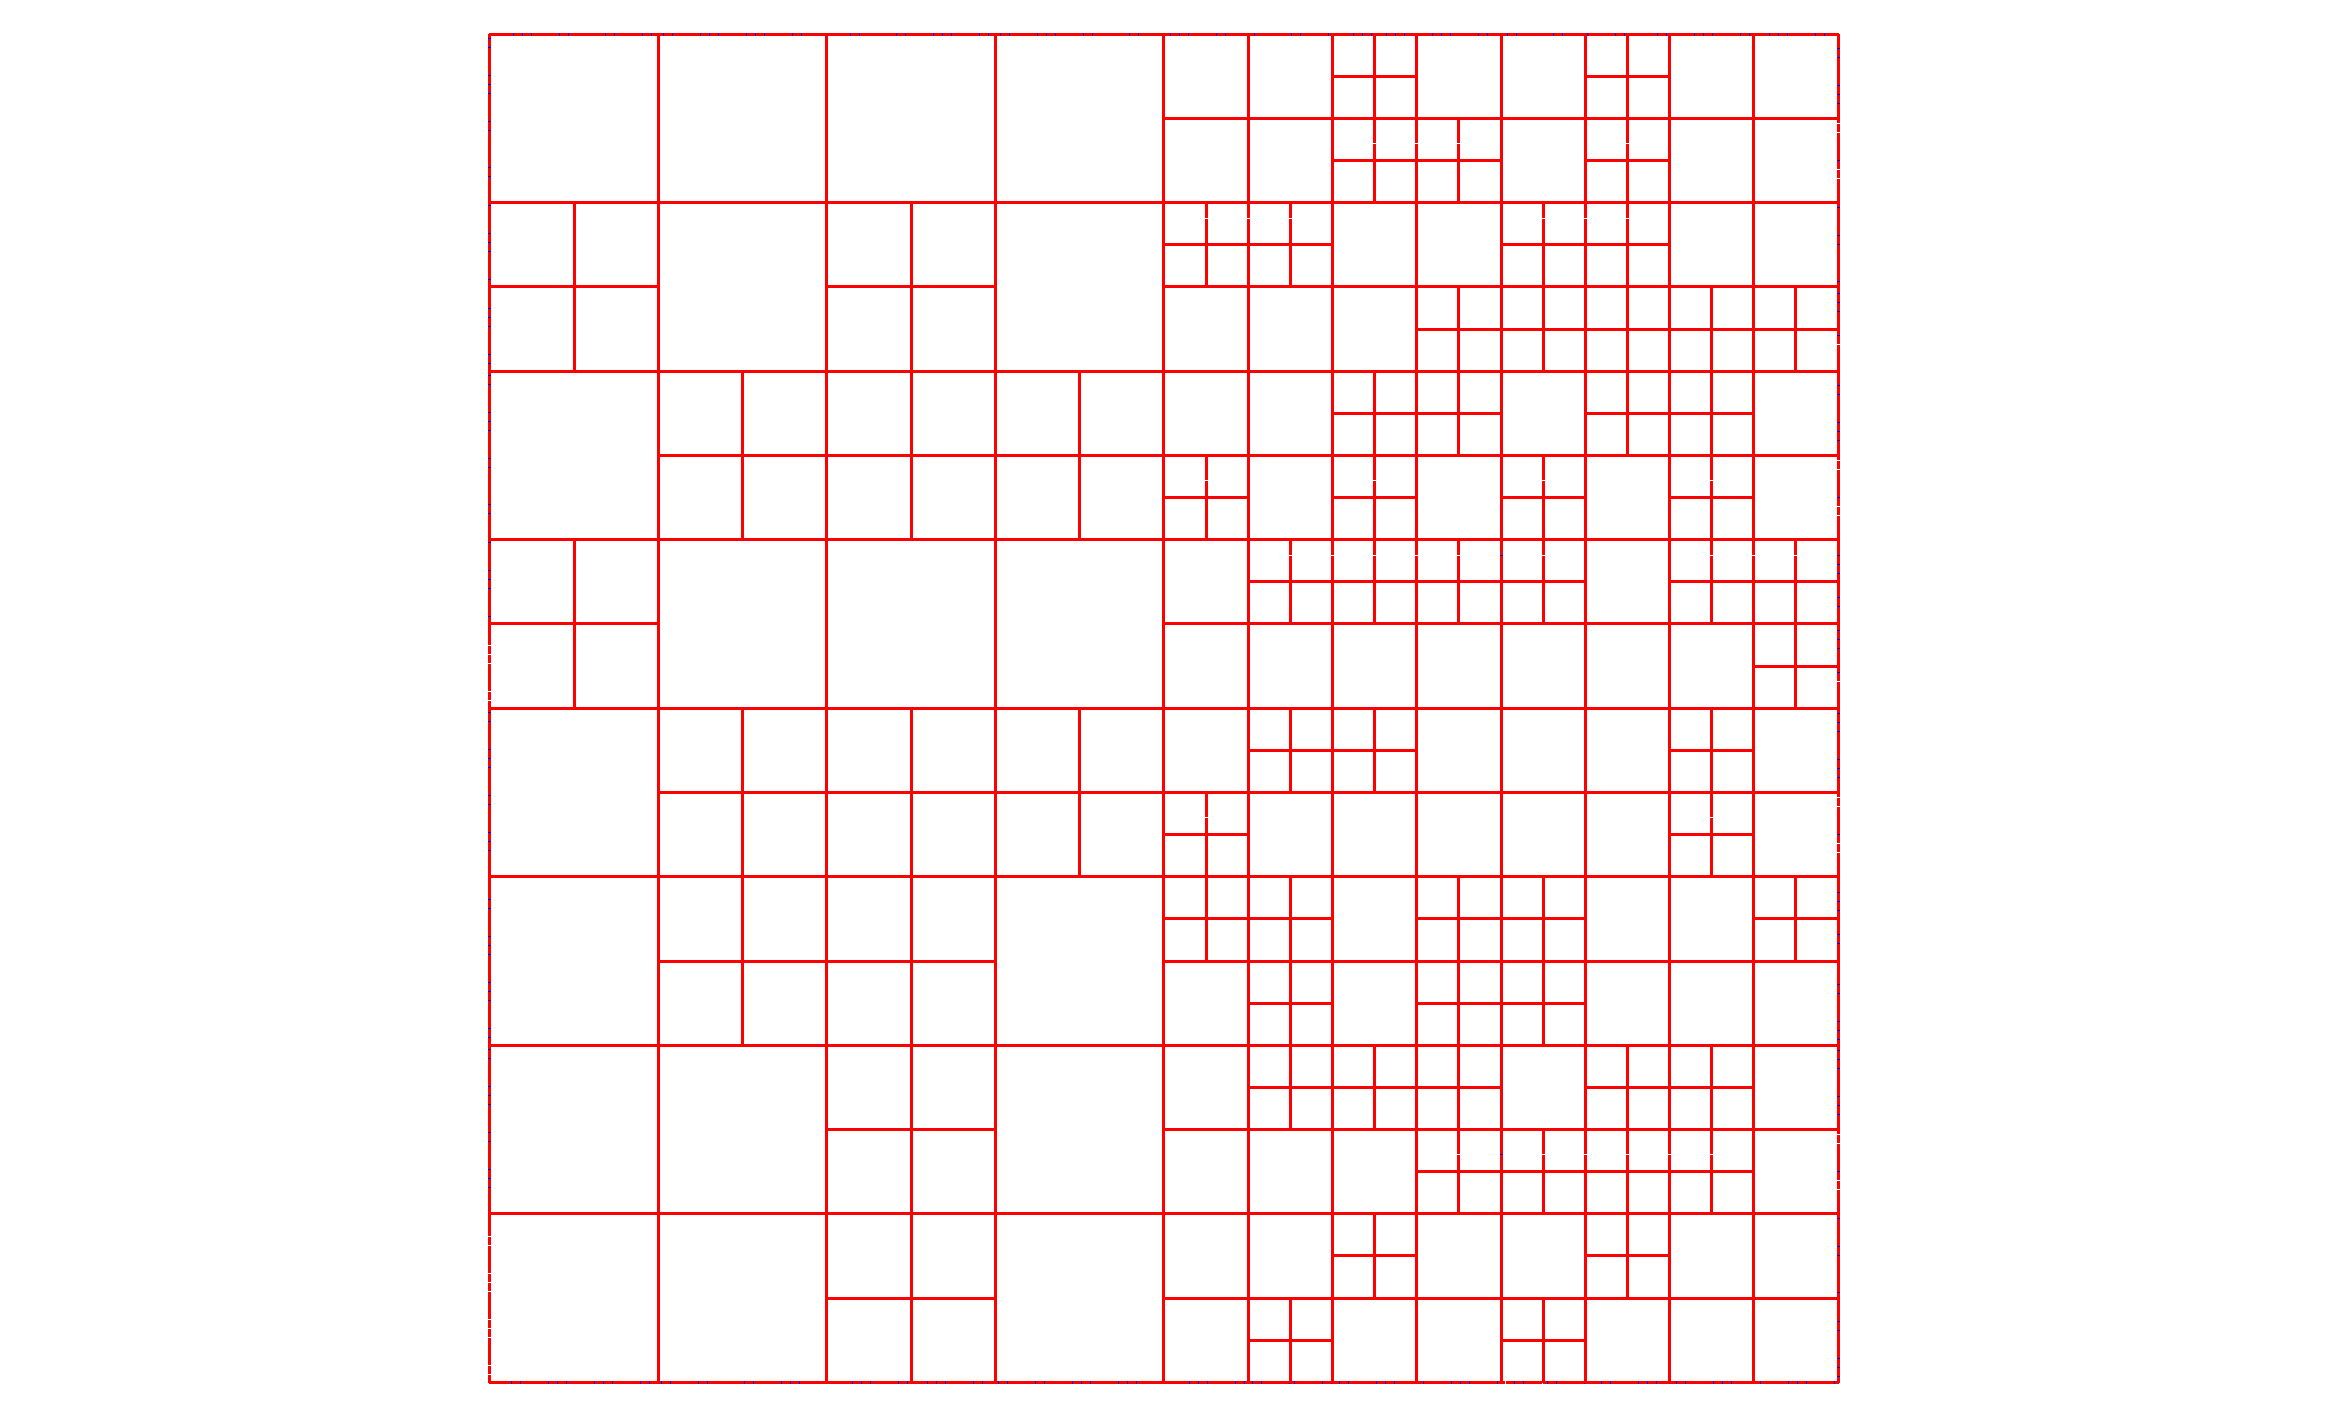
\includegraphics[width=\textwidth]{figures/ByP_Locals}
\end{frame}

\begin{frame}{Solving issues in local quadtree creation}
    \begin{itemize}
        \item Currently working on optimal values for capacity and fraction.
        \item Tradeoff between balance and cost.
    \end{itemize}
\end{frame}

\begin{frame}{Example}{capacity=50, fraction=1}
    \centering
    
\includegraphics[width=\textwidth]{figures/ByC_Globals}
\end{frame}
\begin{frame}{Example}
    \centering
    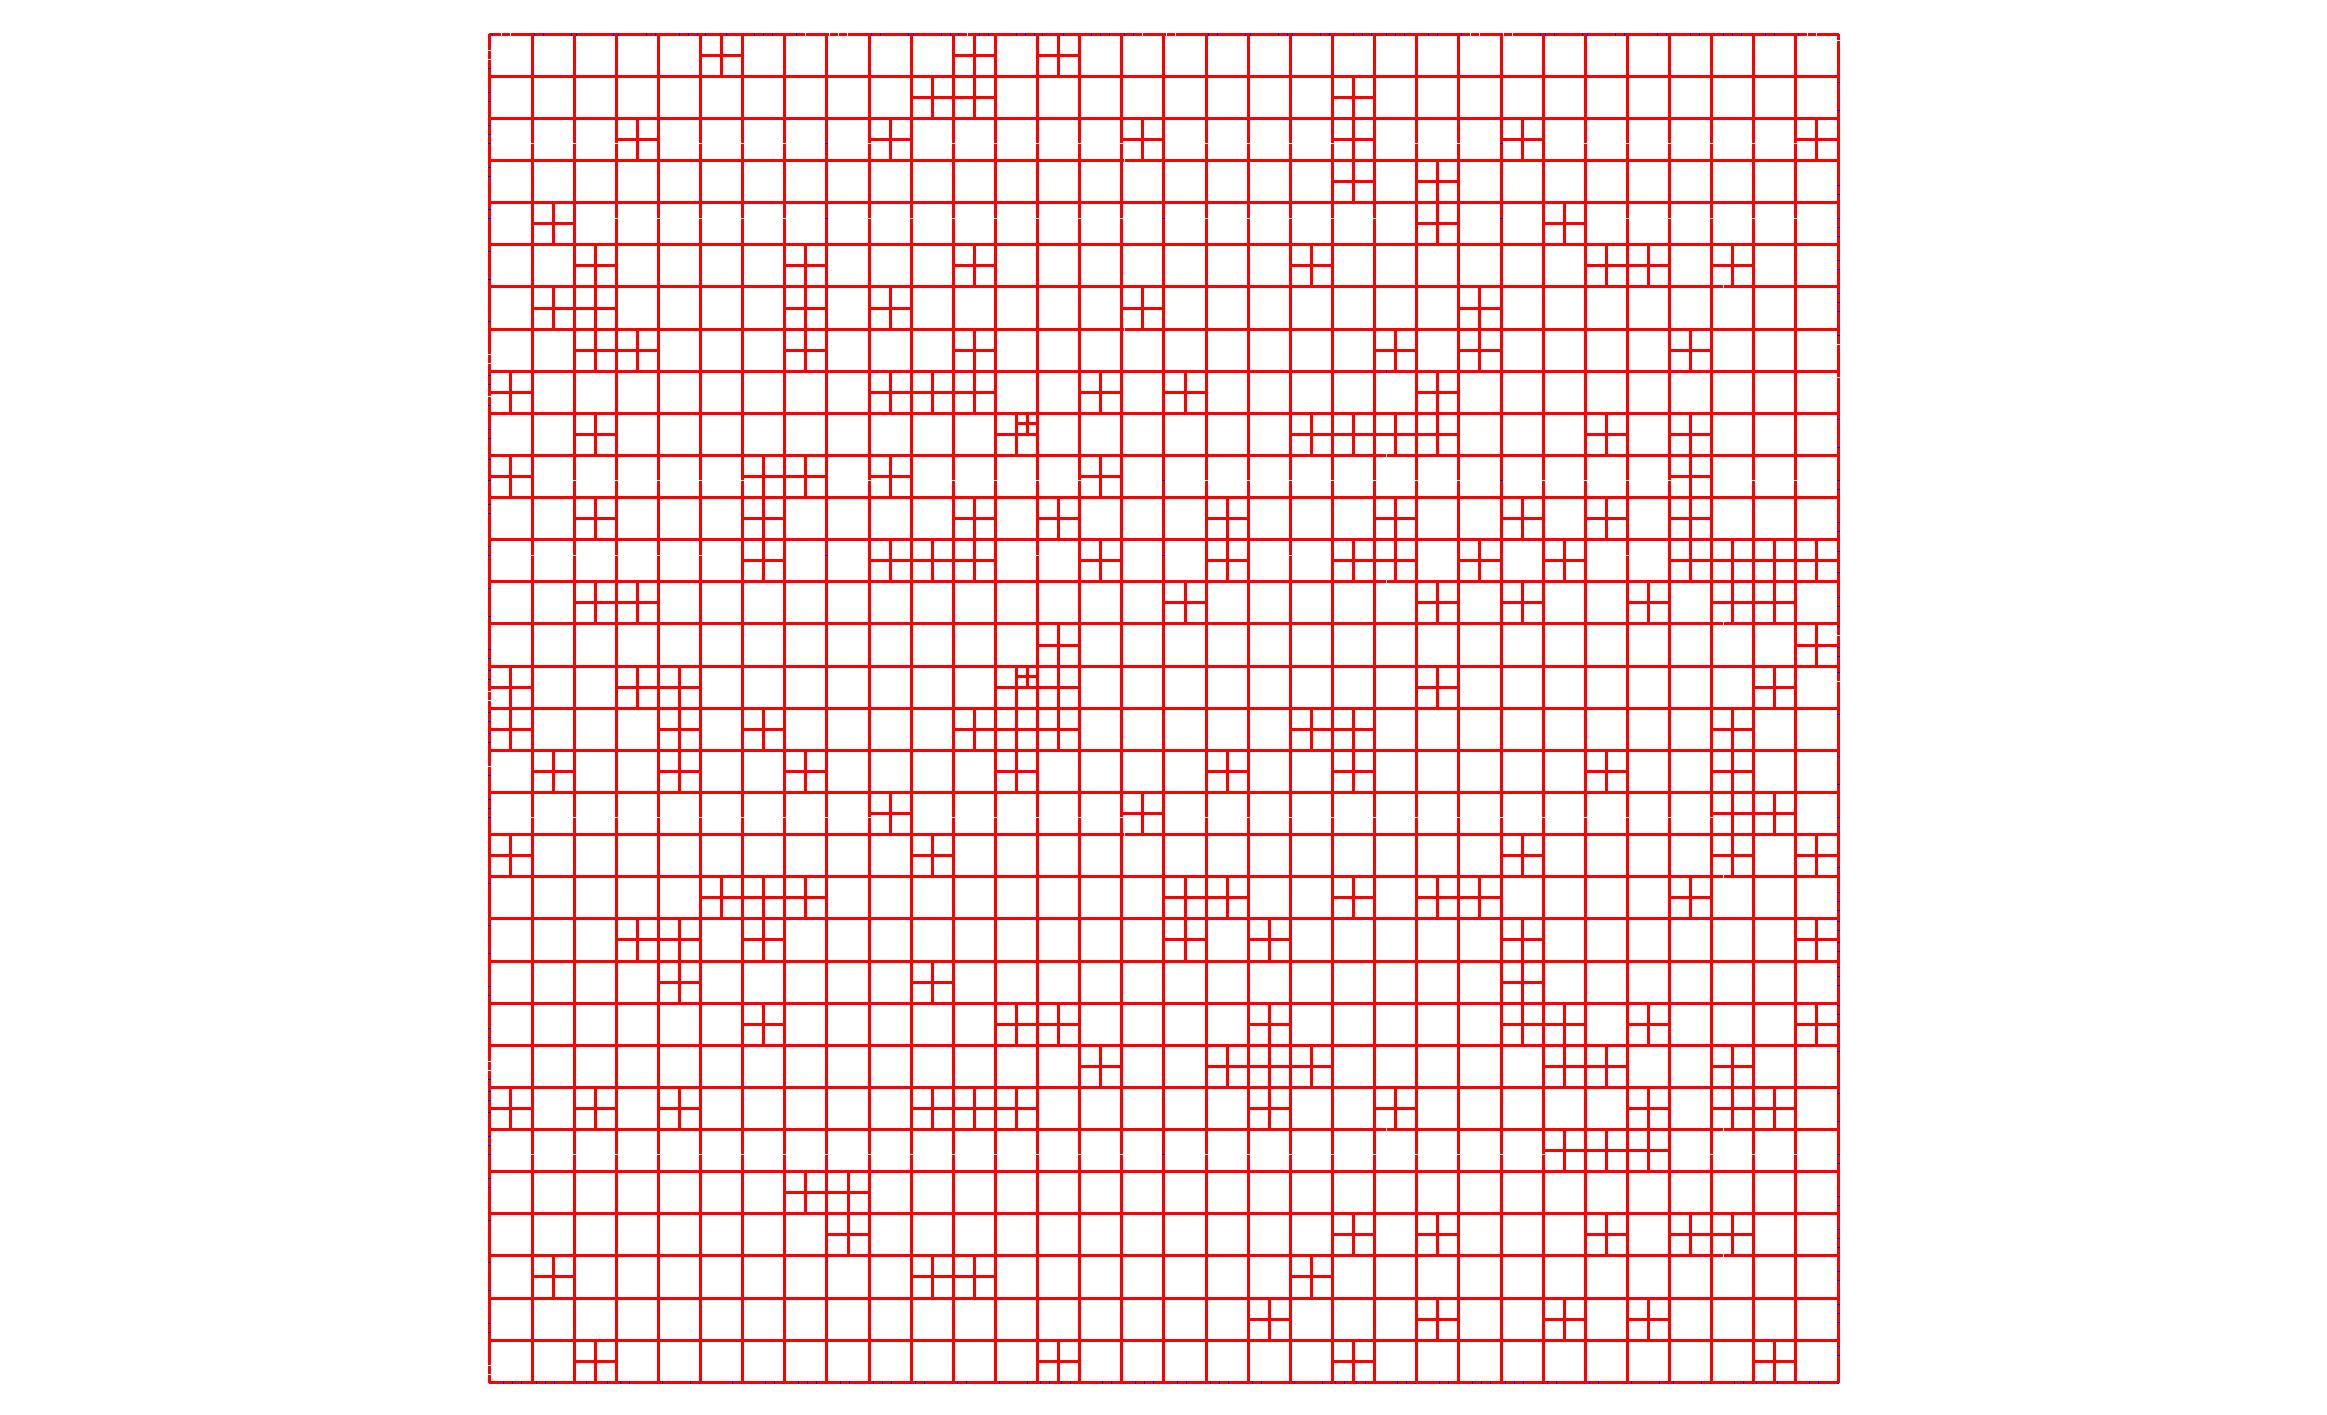
\includegraphics[width=\textwidth]{figures/ByC_Locals}
\end{frame}

\end{document}

